\documentclass[a4paper]{article}
\renewcommand{\contentsname}{tài liệu tham khảo}
\renewcommand{\refname}{tài liêu tham khảo}
\usepackage{listings}
\usepackage{tipa}
\usepackage{amssymb}
\usepackage{color} 
\definecolor{dkgreen}{rgb}{0,0.6,0}
\definecolor{gray}{rgb}{0.5,0.5,0.5}
\definecolor{mauve}{rgb}{0.58,0,0.82}
\usepackage[framemethod=tikz]{mdframed}
\usepackage{alltt}
\usepackage{breakurl}
\usepackage{vntex}
\usepackage{subcaption}
\usepackage{caption}
\DeclareCaptionLabelFormat{cont}{#1~#2\alph{ContinuedFloat}}
\captionsetup[ContinuedFloat]{labelformat=cont}
\usepackage{a4wide,amssymb,epsfig,latexsym,multicol,array,hhline,fancyhdr}
\usepackage{amsmath}
\usepackage{lastpage}
\usepackage[lined,boxed,commentsnumbered]{algorithm2e}
\usepackage{enumerate}
\usepackage{color}
\usepackage{graphicx}							% Standard graphics package
\usepackage{array}
\usepackage{tabularx, caption}
\usepackage{tabu}
\usepackage{multirow}
\usepackage{multicol}
\usepackage{rotating}
\usepackage{graphics}
\usepackage{geometry}
\usepackage{setspace}
\usepackage{float}
\usepackage{epsfig}
\usepackage{tikz}
\usetikzlibrary{arrows,snakes,backgrounds}
\usepackage{hyperref}
\hypersetup{urlcolor=black,linkcolor=black,citecolor=black,colorlinks=true} 
\setlength{\headheight}{40pt}
\pagestyle{fancy}
\fancyhead{} % clear all header fields
\fancyhead[L]{
 \begin{tabular}{rl}
    \begin{picture}(25,15)(0,0)
    \put(0,-8){
\includegraphics[width=8mm, height=8mm]{hcmut.png}}
    %\put(0,-8){\epsfig{width=10mm,figure=hcmut.eps}}
   \end{picture}&
	%
\includegraphics[width=8mm, height=8mm]{hcmut.png} & %
	\begin{tabular}{l}
		\textbf{\bf \ttfamily Trường Đại Học Bách Khoa Tp.Hồ Chí Minh}\\
		\textbf{\bf \ttfamily Khoa Khoa Học và Kỹ Thuật Máy Tính}
	\end{tabular} 	
 \end{tabular}
}
\fancyhead[R]{
	\begin{tabular}{l}
		\tiny \bf \\
		\tiny \bf 
	\end{tabular}  }
\fancyfoot{} % clear all footer fields
\fancyfoot[L]{\scriptsize \ttfamily Báo cáo bài tập lớn}
\fancyfoot[R]{\scriptsize \ttfamily Trang {\thepage}/\pageref{LastPage}}
\renewcommand{\headrulewidth}{0.3pt}
\renewcommand{\footrulewidth}{0.3pt}


%%%
\setcounter{secnumdepth}{4}
\setcounter{tocdepth}{3}
\makeatletter
\newcounter {subsubsubsection}[subsubsection]
\renewcommand\thesubsubsubsection{\thesubsubsection .\@alph\c@subsubsubsection}
\newcommand\subsubsubsection{\@startsection{subsubsubsection}{4}{\z@}%
                                     {-3.25ex\@plus -1ex \@minus -.2ex}%
                                     {1.5ex \@plus .2ex}%
                                     {\normalfont\normalsize\bfseries}}
\newcommand*\l@subsubsubsection{\@dottedtocline{3}{10.0em}{4.1em}}
\newcommand*{\subsubsubsectionmark}[1]{}
\makeatother


\begin{document}

\begin{titlepage}
\begin{center}
ĐẠI HỌC QUỐC GIA THÀNH PHỐ HỒ CHÍ MINH \\
TRƯỜNG ĐẠI HỌC BÁCH KHOA \\
KHOA KHOA HỌC - KỸ THUẬT MÁY TÍNH 
\end{center}

\vspace{1cm}

\begin{figure}[h!]
\begin{center}

\includegraphics[width=3cm]{hcmut.png}
\end{center}
\end{figure}


\vspace{1cm}



\begin{tabular}{l}


\textbf{\Large PHÁT TRIỂN ỨNG DỤNG}\\
\textbf{\Large TRÊN THIẾT BỊ DI ĐỘNG}

\\
\noindent\rule{13cm}{0.4pt}
\\
\\
\Large{Báo cáo bài tập lớn:}\\[2mm]
{\Huge \textbf{ỨNG DỤNG ĐẶT HÀNG}}\\
{\Huge \textbf{TRÊN THIẾT BỊ DI ĐỘNG}}\\
\\
\noindent\rule{13cm}{0.4pt}
\end{tabular}

\vspace{2cm}

\begin{table}[h]
\begin{tabular}{rrll}
\hspace{5 cm} & GVHD: & Trần Công Đời&\\
& & Mai Đức Tú  & 1513924 \\
& & Mai Đức Tú  & 1513924 \\
& & Mai Đức Tú  & 1513924 \\
& & Mai Đức Tú  & 1513924 \\
& & Mai Đức Tú  & 1513924 \\w
\\
\\
\\

\end{tabular}
\end{table}

\begin{center}
{\footnotesize TP. HỒ CHÍ MINH, THÁNG 10/2018}
\end{center}
\end{titlepage}


%\thispagestyle{empty}

\newpage
\tableofcontents

\newpage 
\listoffigures


%%%%%%% GIỚI THIỆU %%%%%%%%%%%%
\newpage
\section{Giới thiệu}
Đưa ứng dụng kỹ thuật công nghệ thông tin vào đời sống đã trở nên phổ biến ở các hình thức trao đổi hàng hoá với khái niệm thương mại điện tử. Chúng ta dần trở nên quen thuộc với các shop bàn hàng hỗ trợ một ứng dụng cho phép đặt hàng online hoặc người bán có thể chỉ là một kho hàng với ứng dụng đặt hàng mà trở thành một shop online. Đó là một hình thức mua bán có nhiều thuận tiện và ngày càng trở nên phổ biến hiện nay. Nắm được nhu cầu đó, nhóm quyết định xây dựng AppOrder cho phép người dùng có thể đặt hàng trên thiết bị di động tới một cửa hàng đã được cấu hình sẵn.
%%%%%%% CẤU TRÚC mã nguồn    %%%%%%%%%%%%
\section{Các tính năng hỗ trợ}
Nhóm xây dựng ứng dụng đặt hàng có đầy đủ chức năng cần thiết cho nhu cầu mua bán thực tế của người dùng. Các tính năng của ứng dụng gồm có:
\begin{enumerate}
    \item Hiển các danh mục sản phẩm category.
    \item Hiển thị danh mục các sản phẩm của từng category.
    \item Hiển thị thông tin chi tiết của sản phẩm.
    \item 
\end{enumerate}
\section{Cấu trúc mã nguồn}
\subsection{Thư mục page}
Thông tin chi tiết của các tập tin trong thư mục \textbf{page} gồm các file HTML như sau:

\begin{itemize}
    \item about.html: Trang thông tin chung của website và thành viên
    \item category.html: Trang trình bày các mẫu template phân theo danh mục
    \item details.html: Trang thông tin chi tiết của từng mẫu template 
    \item home.html: Trang chủ của website có mục đích tạo ấn tượng và hướng dẫn cho người dùng
    \item login.html: Trang dành cho khách hàng đăng nhập vào tài khoản online
    \item product.html: Trang sản phẩm sắp xếp theo các tiêu chí như yêu thích nhất, nhiều lượt tải nhất ...
    \item signup.html: Trang dành cho khách hàng đăng ký tài khoản mới
\end{itemize}

\subsection{Thư mục css}
Thông tin chi tiết của các tập tin trong thư mục CSS như sau:

\begin{itemize}
    \item themes: thư mục con chứa các assets như font, ảnh
    \item common.css: các thông số chung cho các page
    \item sematic.css: các thông số của framework hỗ trợ mà nhóm sử dụng
    \item *.css còn lại: chứa thông số hỗ trợ cho từng trang html tương ứng ở thư mục page, ví dụ home.css hỗ trợ cho home.html
\end{itemize}

\subsection{Thư mục js}
Thư mục này chứa các file javascript cần thiết để xây dựng các chức năng cho website.
\begin{itemize}
    \item angular.min.js, anime.js, particle.js, sematic.js: chứa các hàm hiệu ứng có sẵn của framework.
    \item *.js còn lại: chứa các hàm hiệu ứng hỗ trợ cho từng trang html tương ứng ở thư mục page, ví dụ home.js hỗ trợ cho home.html
\end{itemize}

\subsection{Thư mục assets, bootstrap, components}
Các thư mục hỗ trợ hiệu ứng của framework
%%%%%%% CẤU TRÚC WEBSITE %%%%%%%%%%%%


\subsection{Trang thông tin web}
Trang thông tin web được xây dựng và hiện thực ở file \texttt{about.html}. Phầnn nội dung của Trang thông tin web bao gồm các phần sau:
\begin{itemize}
    \item Mục nội dung giới thiệu.
    \item Hình ảnh thêm sinh động cho mục tương ứng.
\end{itemize}
Ở các màn hình lớn, nội dung và hình ảnh sẽ ở hai cột song song. Khi chuyển sang màn hình nhỏ, nội dung và hình ảnh sẽ xen kẽ nhau ở một cột.

\subsection{Trang danh mục}
Trang danh mục được xây dựng và hiện thực ở file \texttt{category.html}. Phần nội dung của Trang danh mục bao gồm các phần sau:
\begin{itemize}
    \item Sidebar nằm ở bên trái để lựa chọn các mục templates khác nhau
    \item Nội dung là các template có kèm ảnh minh hoạ và nút review để chuyển sang trang chi tiết.
\end{itemize}

\subsection{Trang chi tiết}
Trang chi tiết được xây dựng và hiện thực ở file \texttt{details.html}. Phần nội dung của Trang chi tiết bao gồm các phần sau:
\begin{itemize}
    \item Các ảnh demo của template
    \item Thông tin mô tả template
    \item Nút "Download", nút "Review" giành cho website có thể demo online
    \item Mục chia sẻ có các nút tương ứng liên kết với các mạng xã hội khác nhau
    \item Mục comment của khách hàng
    \item Mục các sản phẩm liên quan
\end{itemize}

\subsection{Trang chủ}
Trang chủ được xây dựng và hiện thực ở file \texttt{home.html}. Phần nội dung của Trang chủ bao gồm các phần sau:
\begin{itemize}
    \item Màn hình nền ấn tượng người xem
    \item Nút "Start" kích hoạt giao diện hướng dẫn người dùng
    \item Nút "Next" di chuyển giữa các trang hướng dẫn sau khi sử dụng nút "Start"
    \item Nút "Home" sau khi người dùng đã xem hết các trang hướng dẫn
    \item Các hiện ứng màu sắc
\end{itemize}

\subsection{Trang đăng nhập}
Trang đăng nhập được xây dựng và hiện thực ở file \texttt{login.html}. Phần nội dung của Trang đăng nhập bao gồm các phần sau:
\begin{itemize}
    \item Vùng điền tên tài khoản "username" của khách hàng 
    \item Vùng điền mật khẩu "password" của khách hàng
    \item Nút "remember me" nhớ người dùng cho lần đăng nhập tiếp theo
    \item Nút đăng nhập "Login".
    \item Nút tạo tài khoản mới "Sign up"
\end{itemize}

\subsection{Trang sản phẩm}
Trang sản phẩm được xây dựng và hiện thực ở file \texttt{product.html}. Phần nội dung của Trang sản phẩm bao gồm các phần sau:
\begin{itemize}
    \item Mục các mẫu yêu thích
    \item Mục các mẫu Web
    \item Mục các mẫu trình chiếu 
\end{itemize}

\subsection{Trang đăng ký}
Trang đăng ký được xây dựng và hiện thực ở file \texttt{signup.html}. Phần nội dung của Trang đăng ký bao gồm các phần sau:
\begin{itemize}
    \item Vùng điền tên tài khoản "user name" của khách hàng 
    \item Vùng điền địa chỉ thư điện tử "email" của khách hàng 
    \item Vùng điền mật khẩu "password" của khách hàng
    \item Vùng điền lặp lại mật khẩu "repeat password" của khách hàng
    \item Nút nhớ đồng ý điều khoản của website "I agree to the terms and conditions"
    \item Nút đăng ký "Sign up"
    \item Nút đăng nhập "login"
\end{itemize}


%%%%%%% ẢNH CHỤP MÀN HÌNH %%%%%
\newpage
\section{Ảnh chụp màn hình}
\subsection{Hiển thị trên Chrome}

\begin{figure}[H]
\begin{center}
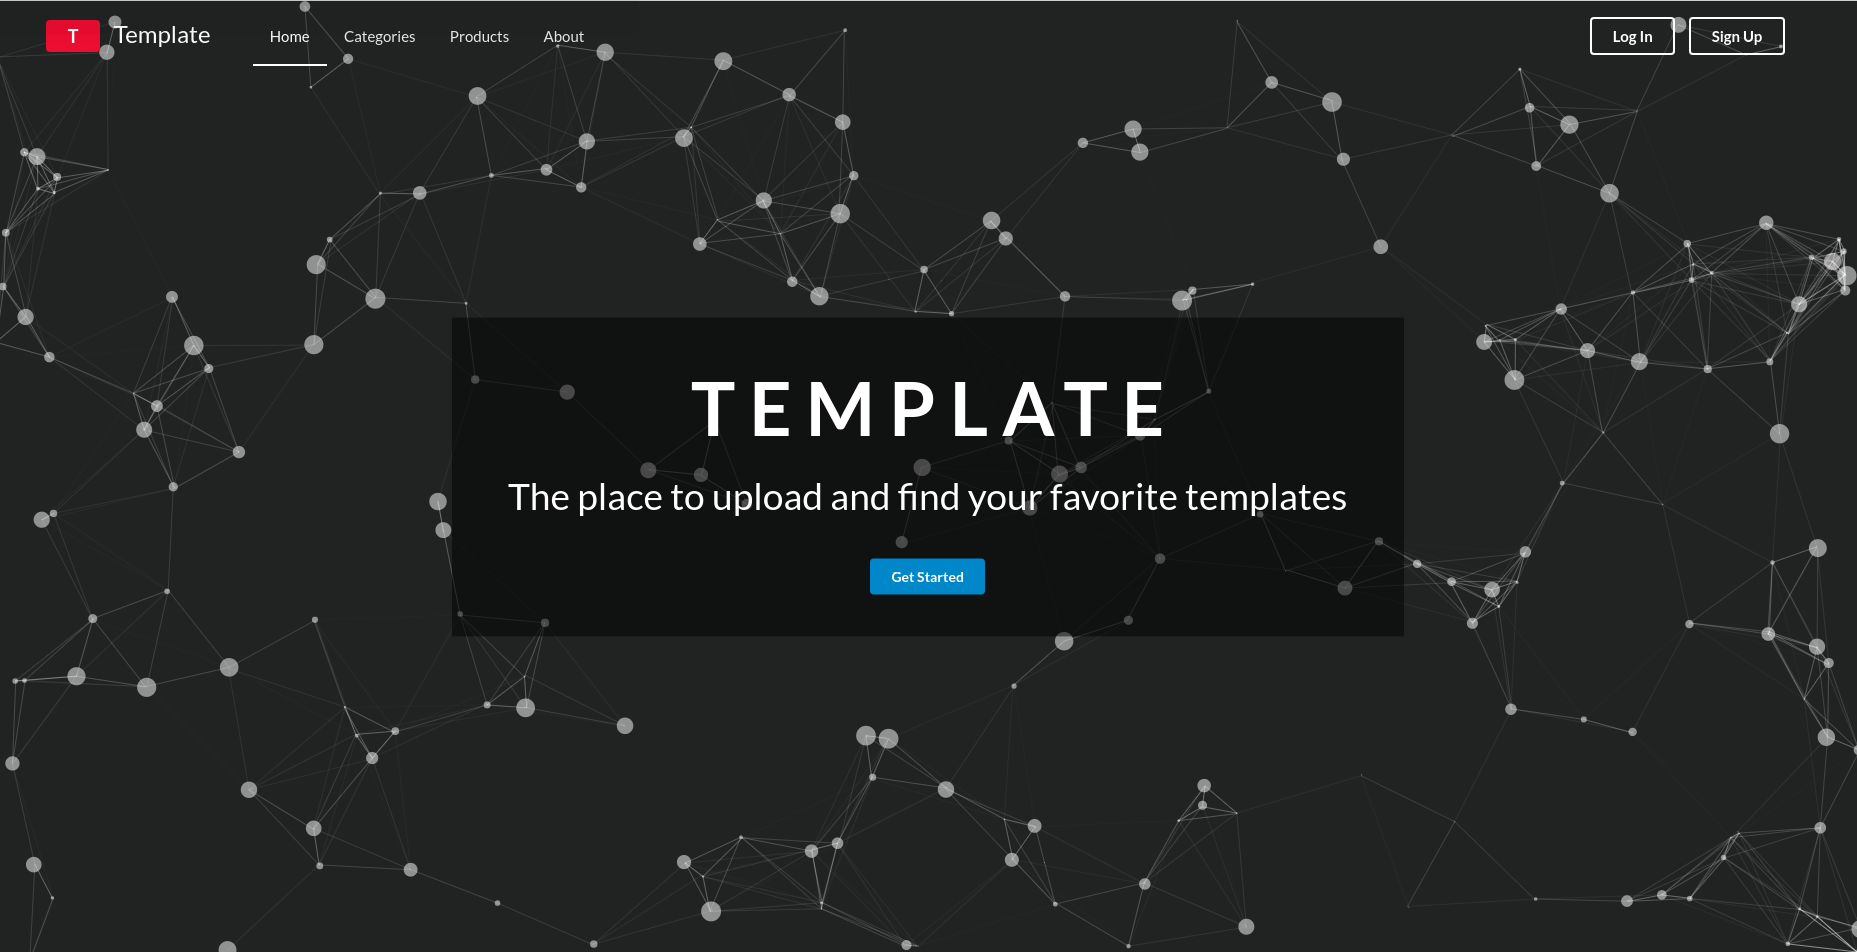
\includegraphics[page=1, scale=0.215]{screenshot/chrome1.png}
\caption{Ảnh chụp trang home.html trên chrome browser}
\end{center}
\end{figure}

\begin{figure}[H]
\begin{center}
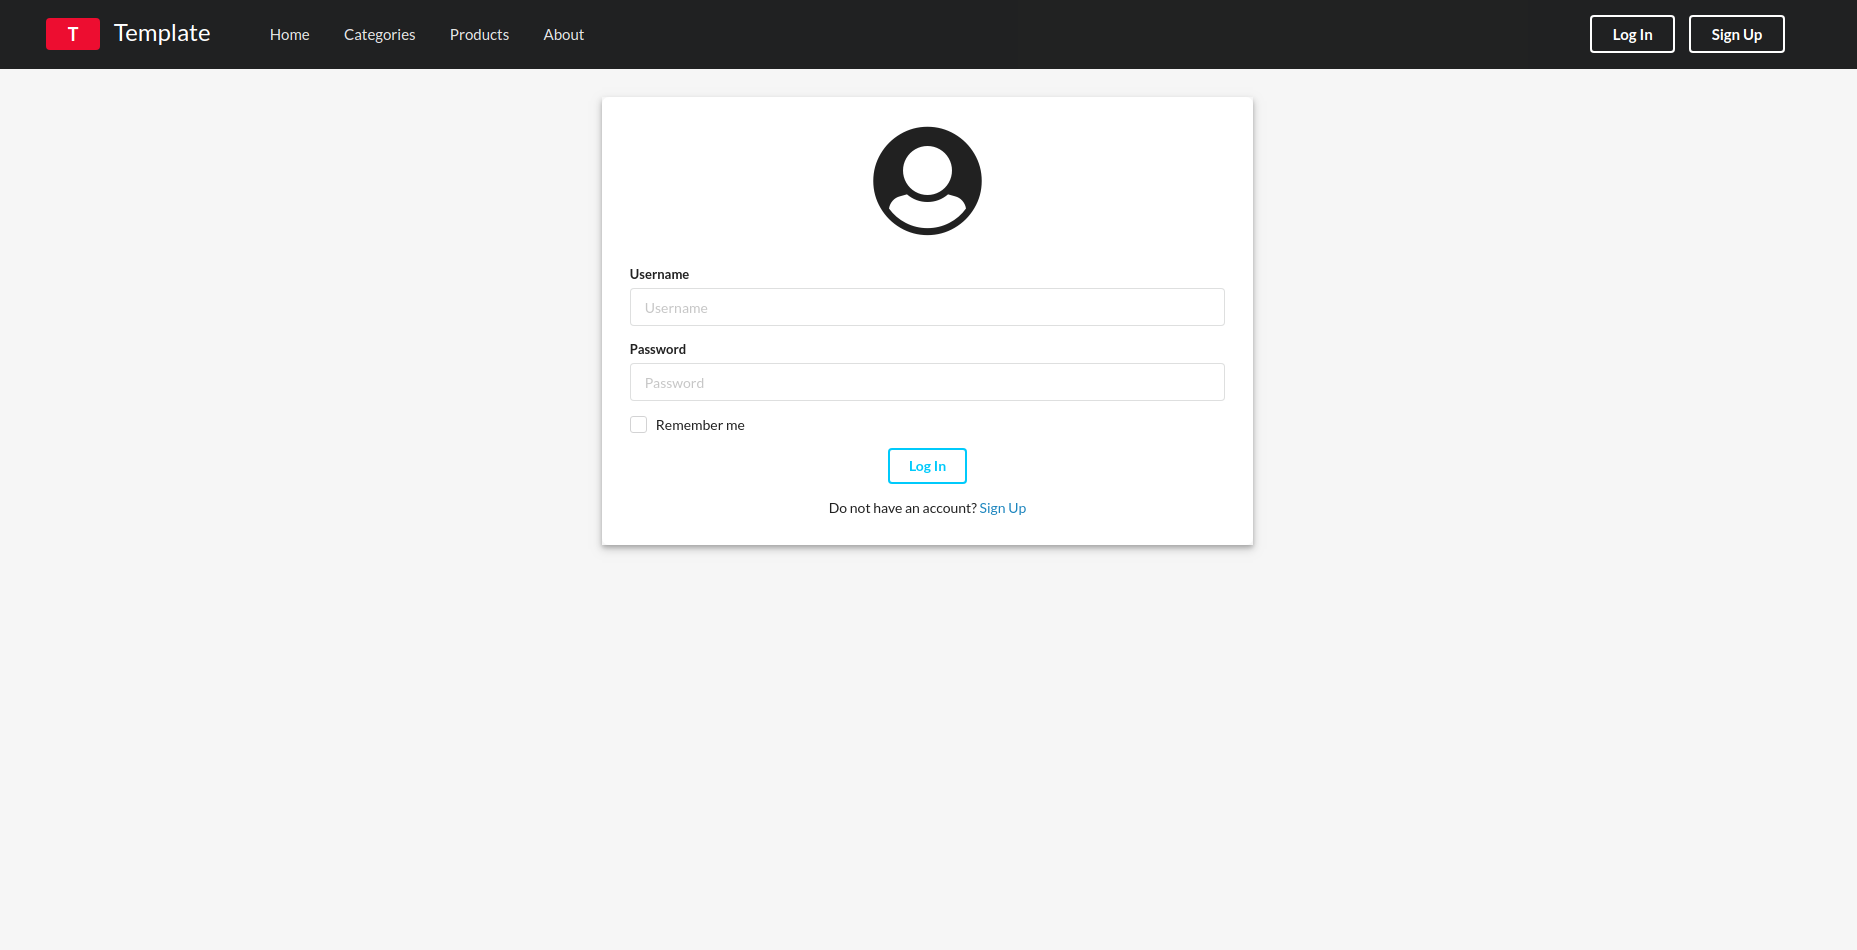
\includegraphics[page=1, scale=0.215]{screenshot/chrome2.png}
\caption{Ảnh chụp trang login.html trên chrome browser}
\end{center}
\end{figure}

\begin{figure}[H]
\begin{center}
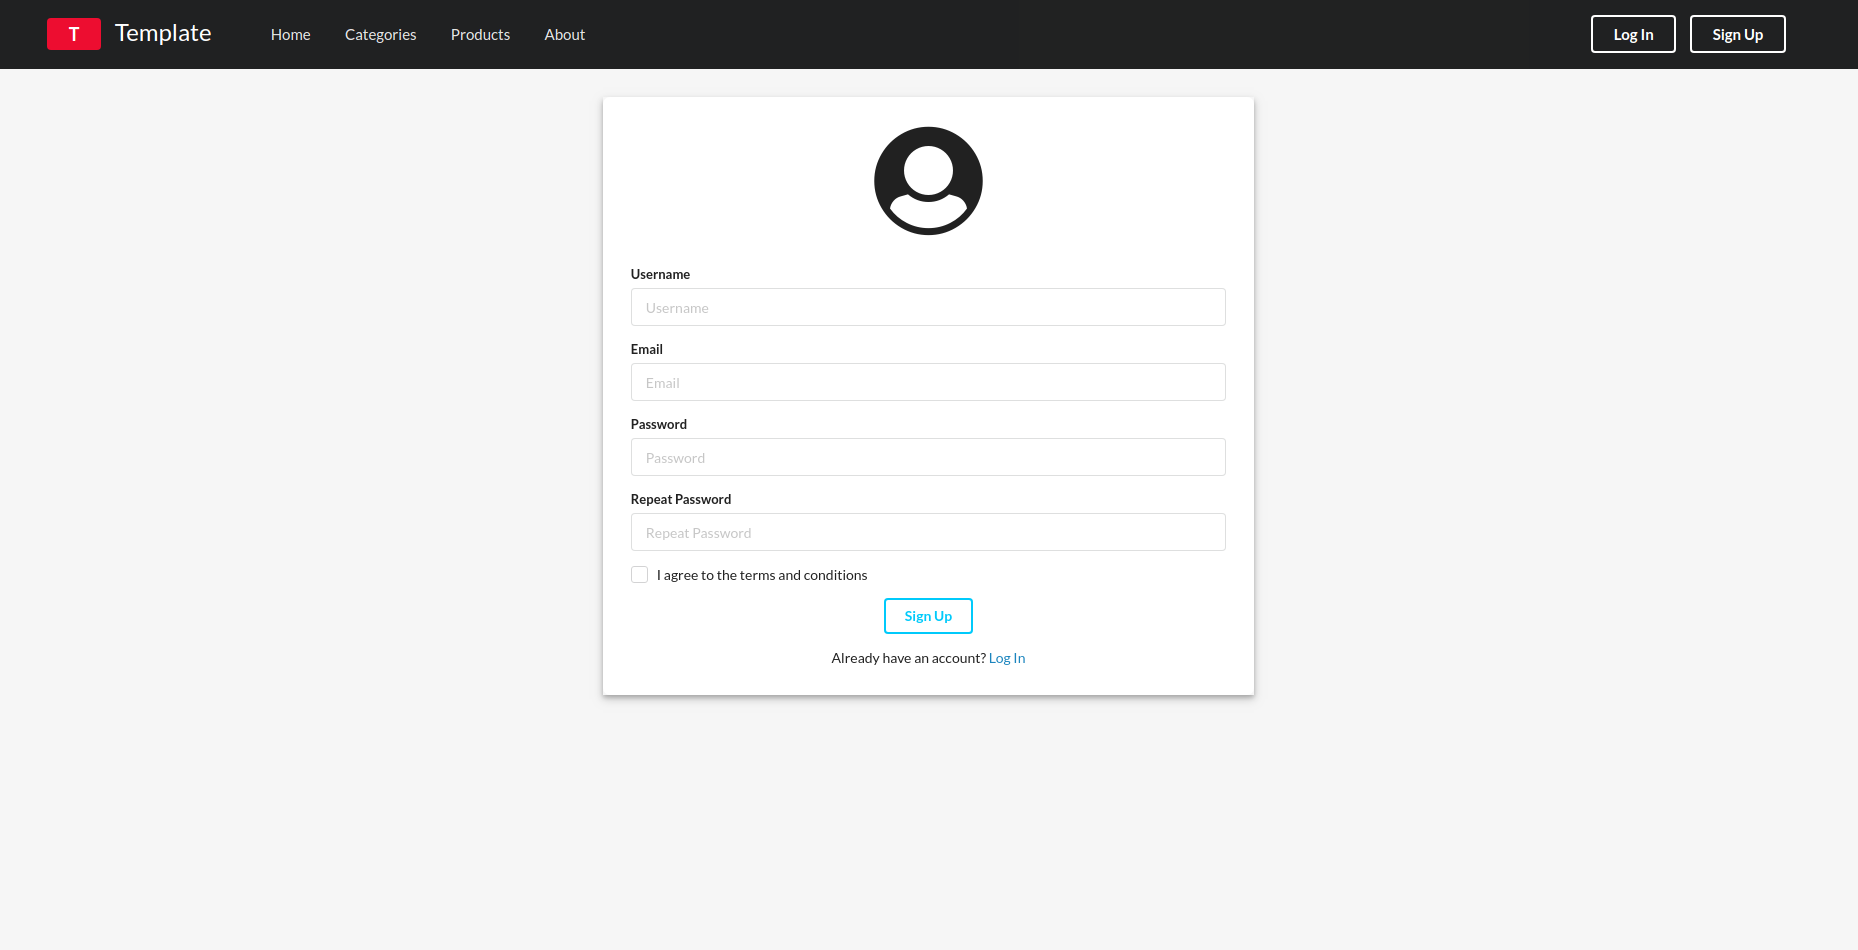
\includegraphics[page=1, scale=0.215]{screenshot/chrome3.png}
\caption{Ảnh chụp trang signup.html trên chrome browser}
\end{center}
\end{figure}

\begin{figure}[H]
\begin{center}
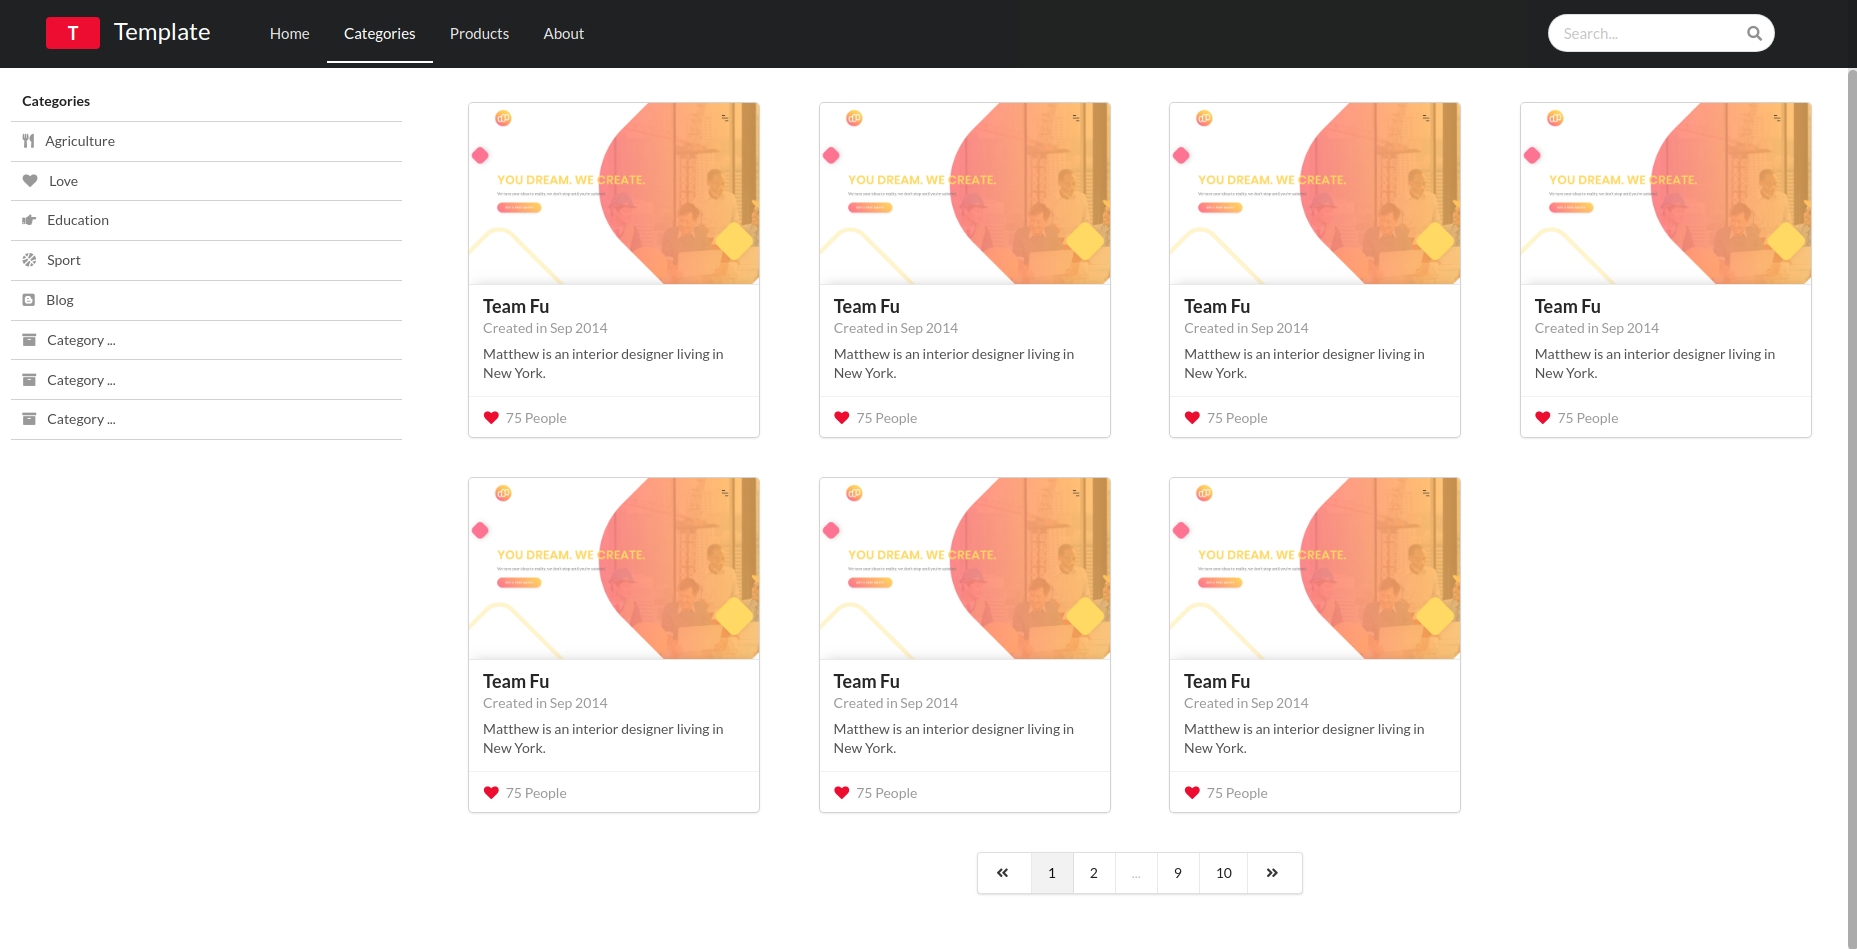
\includegraphics[page=1, scale=0.215]{screenshot/chrome4.png}
\caption{Ảnh chụp trang category.html trên chrome browser}
\end{center}
\end{figure}

\begin{figure}[H]
\begin{center}
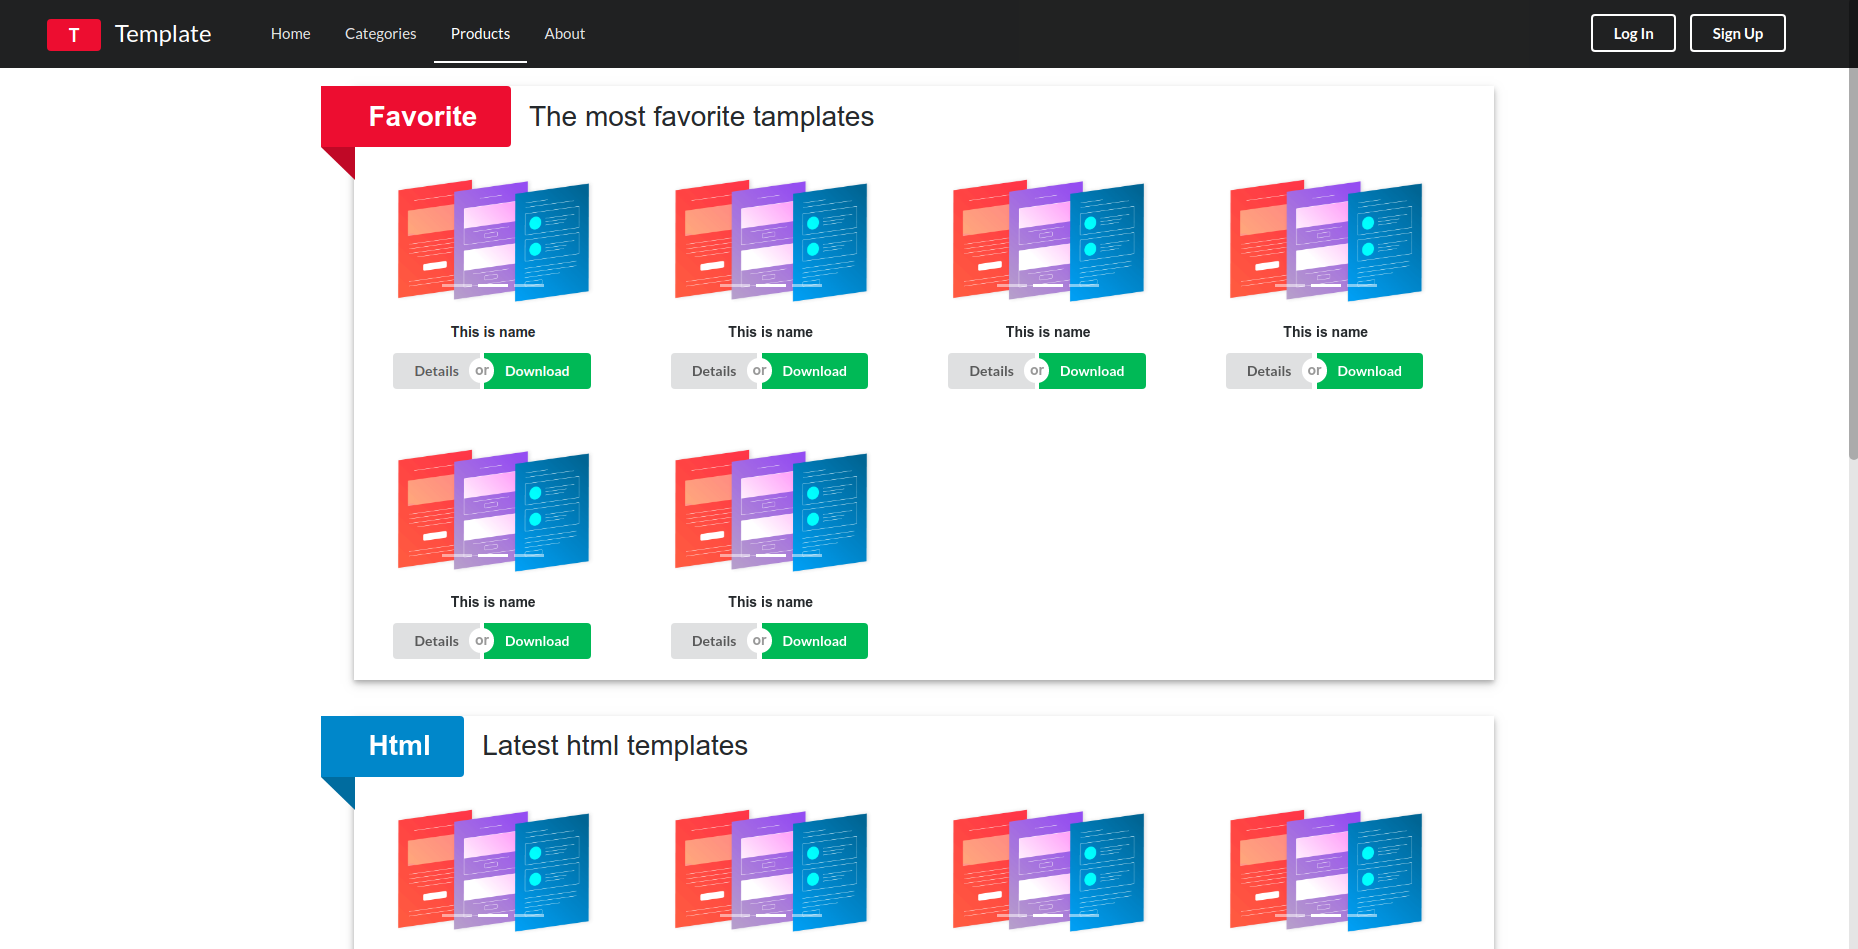
\includegraphics[page=1, scale=0.215]{screenshot/chrome5.png}
\caption{Ảnh chụp trang product.html trên chrome browser}
\end{center}
\end{figure}

\begin{figure}[H]
\begin{center}
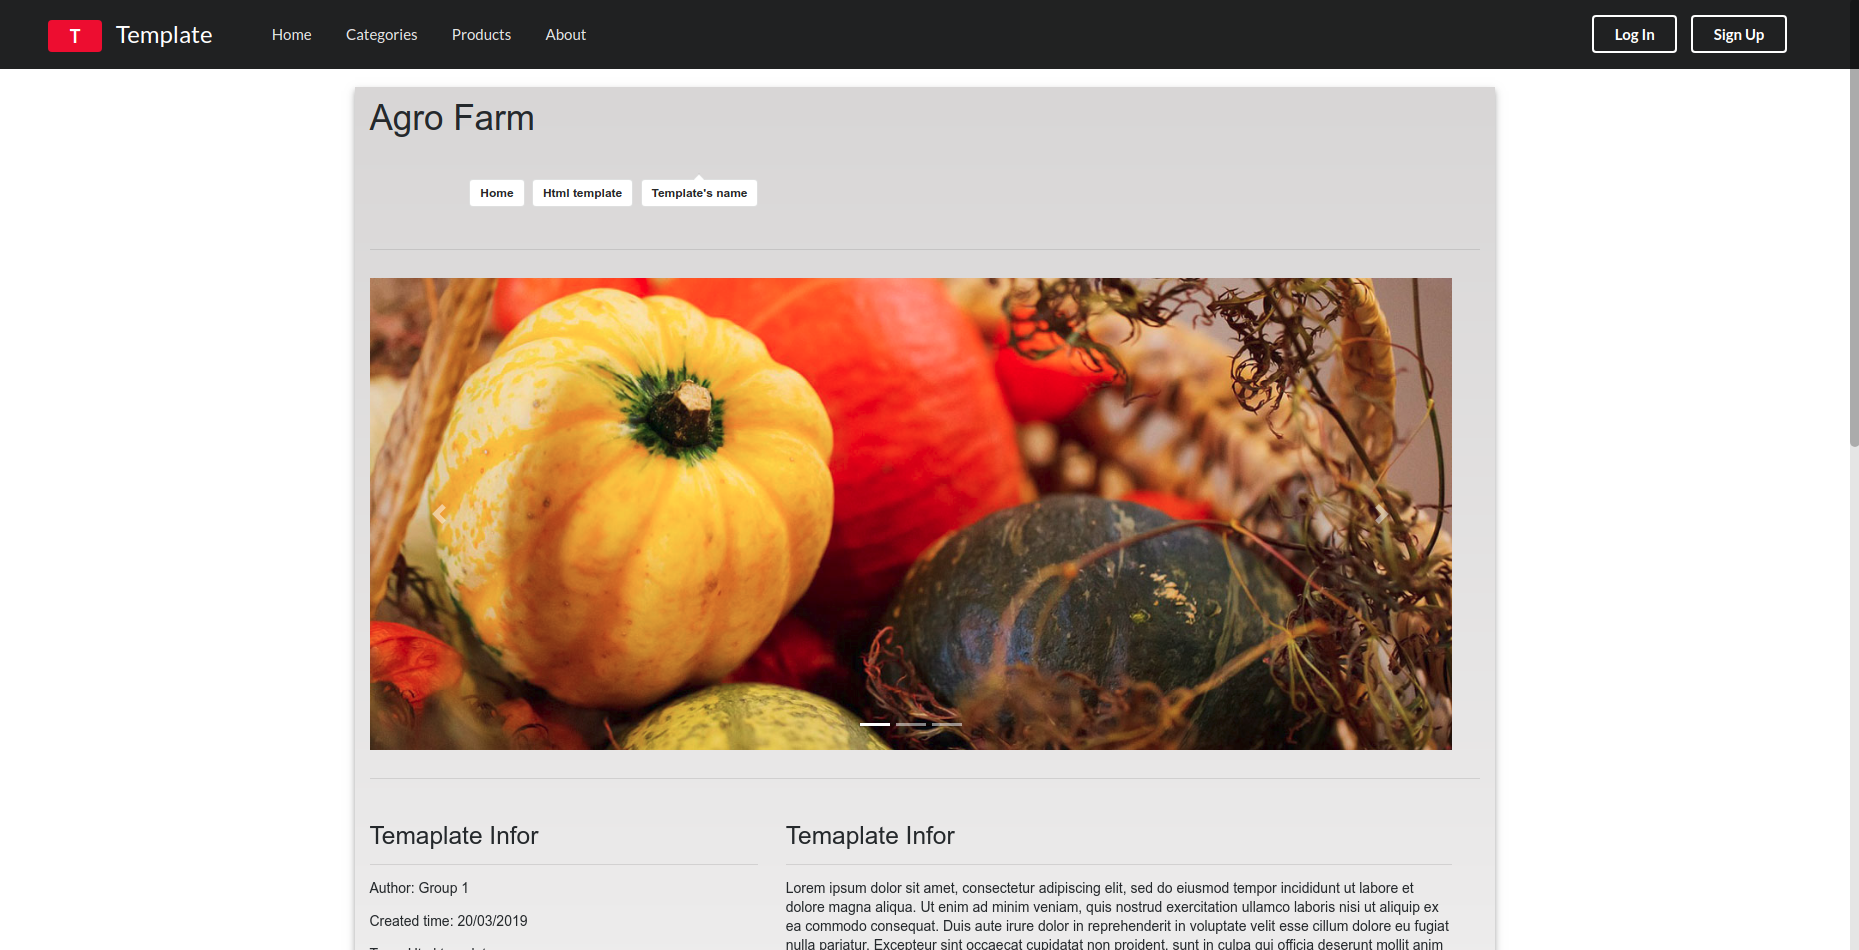
\includegraphics[page=1, scale=0.215]{screenshot/chrome6.png}
\caption{Ảnh chụp trang details.html trên chrome browser}
\end{center}
\end{figure}

\begin{figure}[H]
\begin{center}
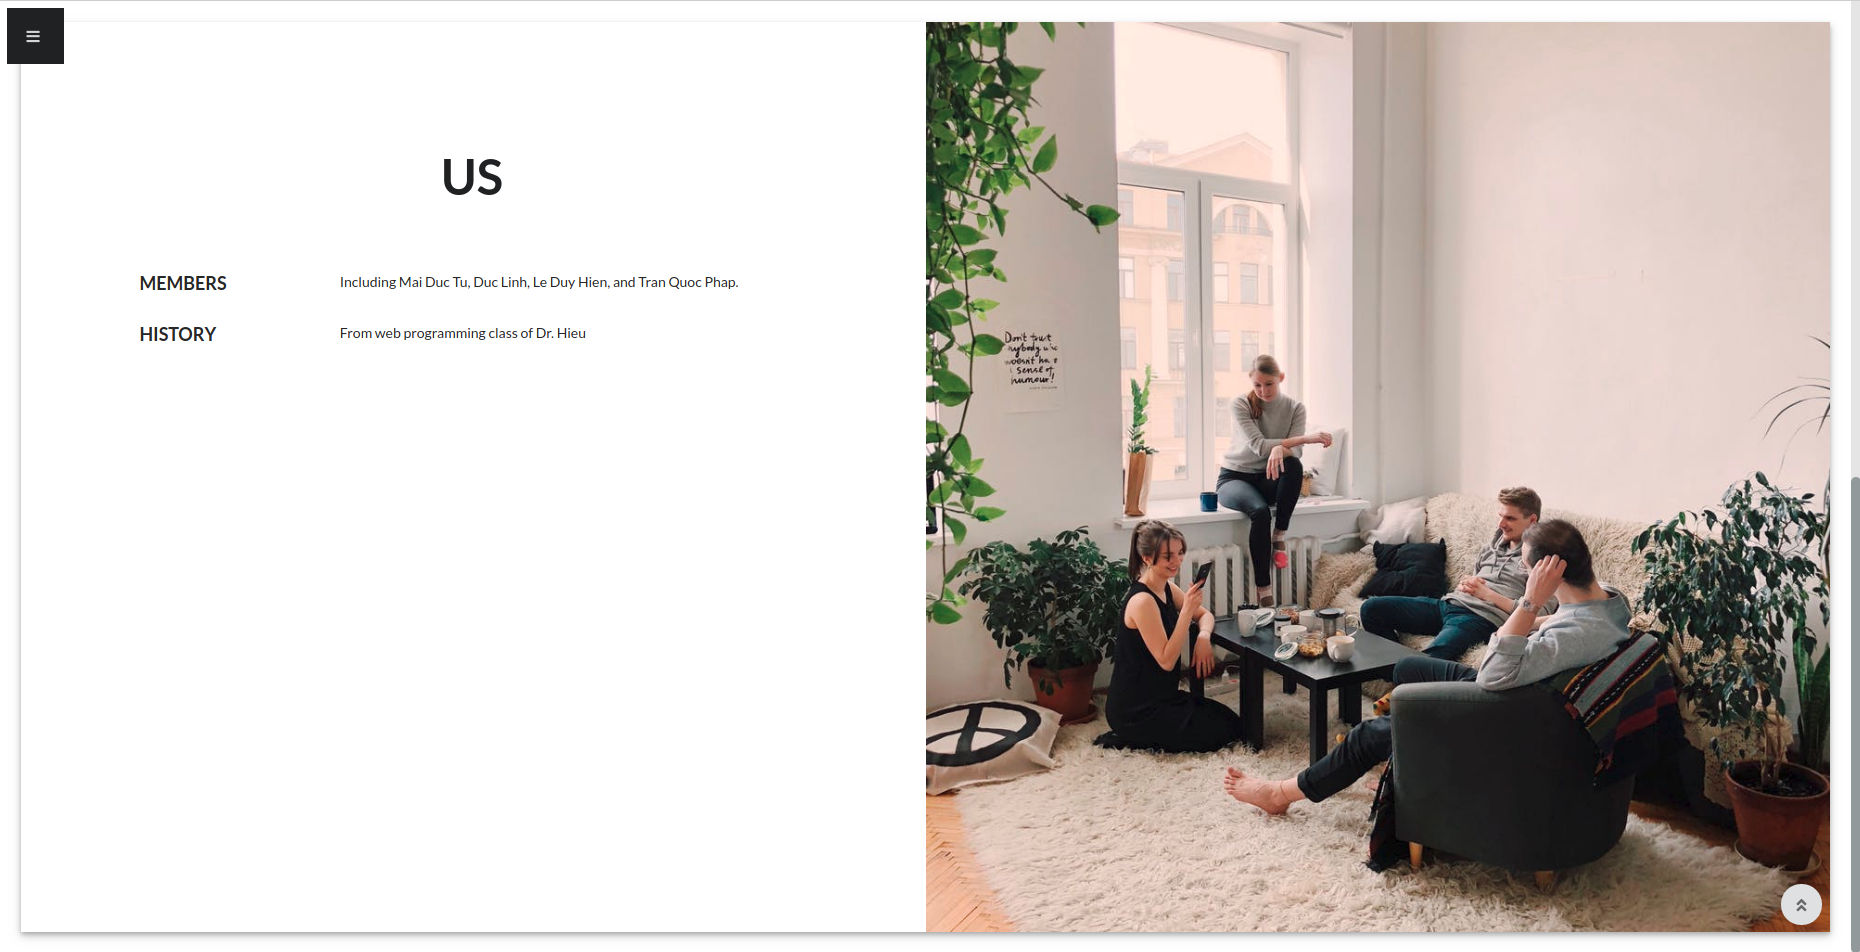
\includegraphics[page=1, scale=0.215]{screenshot/chrome7.png}
\caption{Ảnh chụp trang about.html trên chrome browser}
\end{center}
\end{figure}

% % microsoft edge
% \subsection{Hiển thị trên Microsoft Edge}
% \begin{figure}[H]
% \begin{center}
% \includegraphics[page=1, scale=0.36]{screenshot/edge1.png}
% \caption{Ảnh chụp giao diện trang gop\_y.html trên Microsoft Edge}
% \end{center}
% \end{figure}

% \begin{figure}[H]
% \begin{center}
% \includegraphics[page=1, scale=0.36]{screenshot/edge2.png}
% \caption{Ảnh chụp giao diện trang chi\_tiet\_truyen.html trên Microsoft Edge}
% \end{center}
% \end{figure}


% fire fox


\begin{figure}[H]
\begin{center}
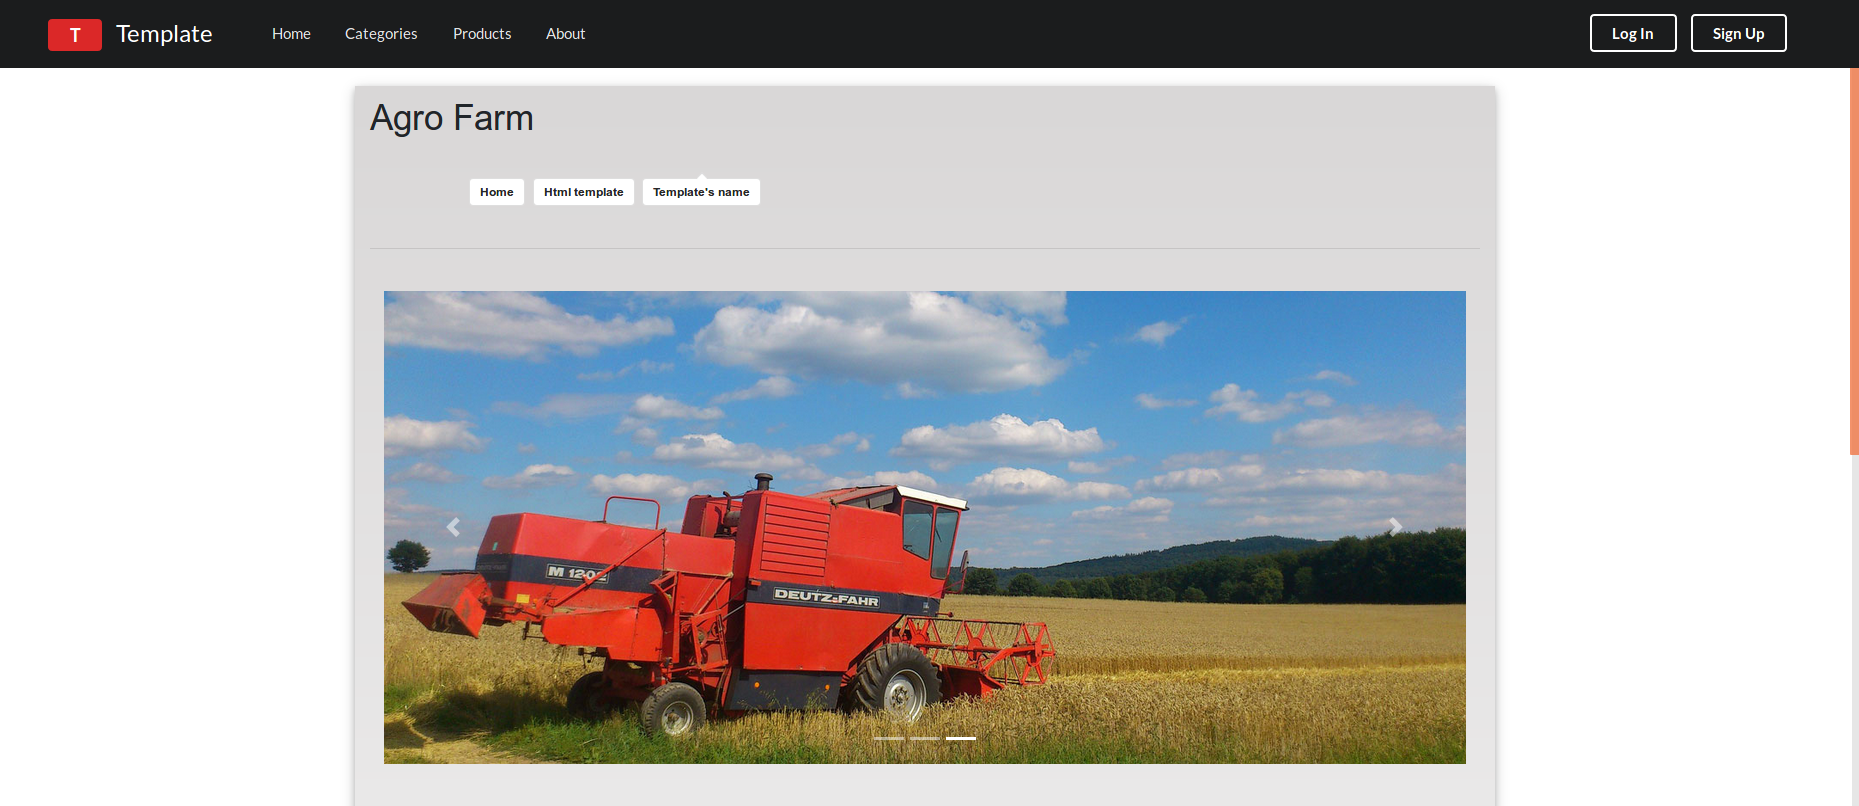
\includegraphics[page=1, scale=0.215]{screenshot/firefox2.png}
\caption{Ảnh chụp trang details.html phần header và slide trên Firefox browser}
\end{center}
\end{figure}


\begin{figure}[H]
\begin{center}
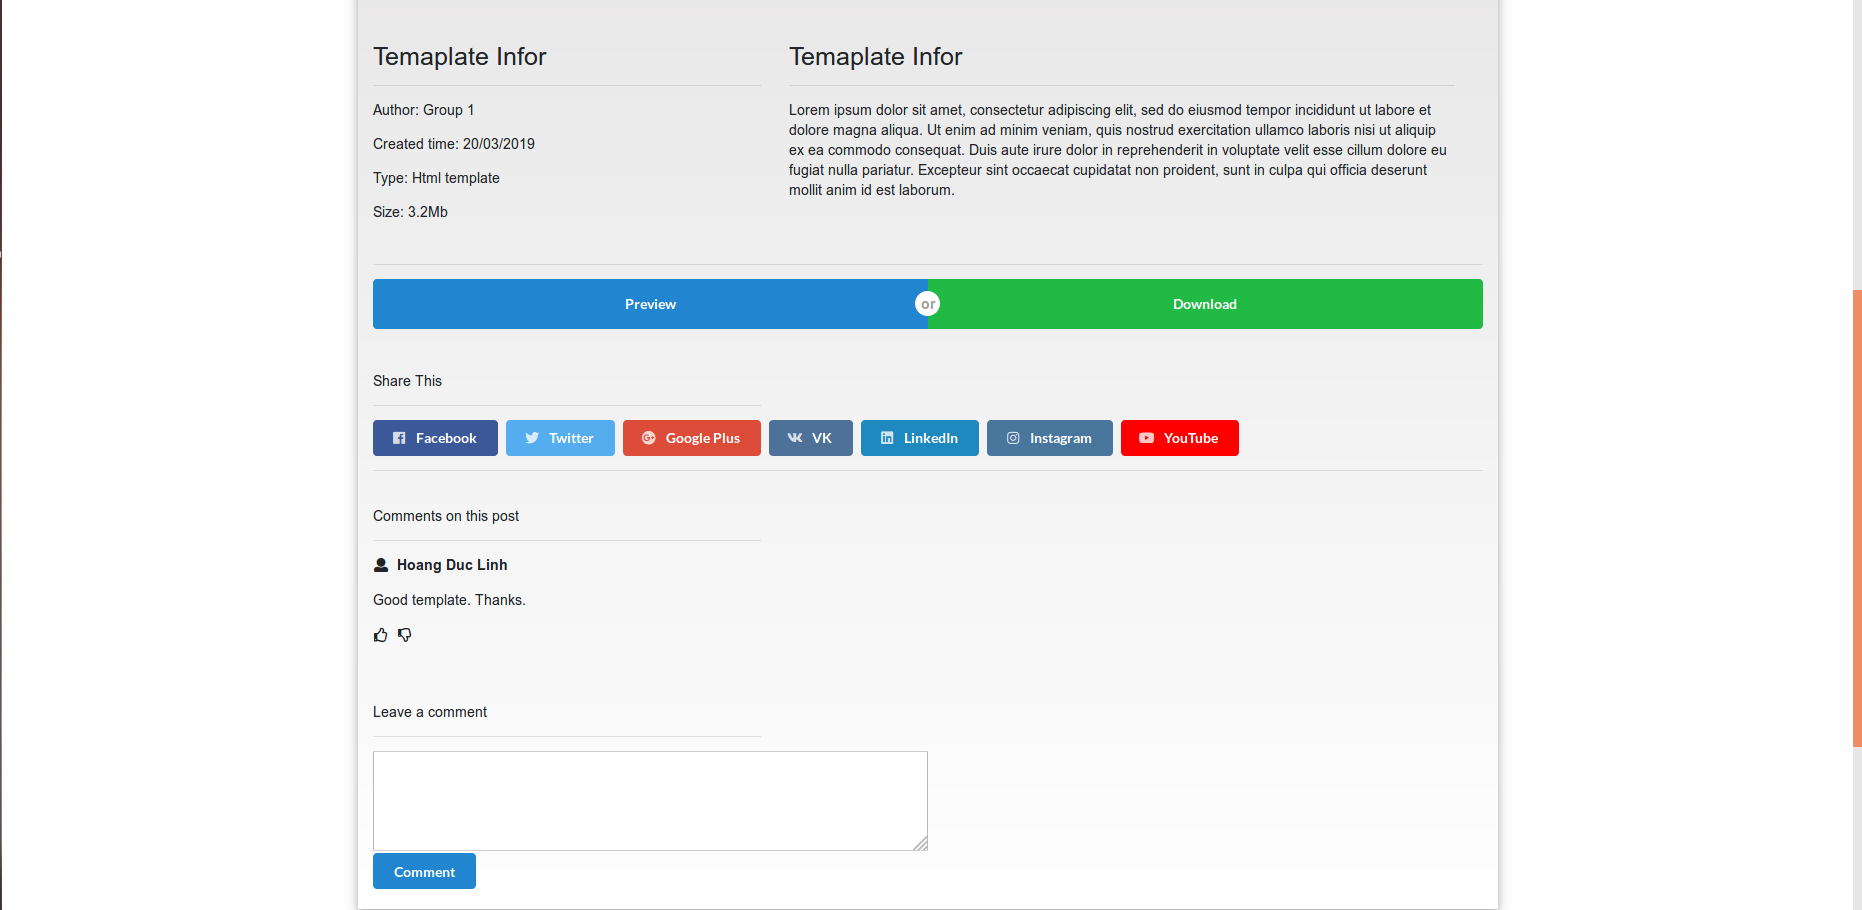
\includegraphics[page=1, scale=0.215]{screenshot/firefox3.png}
\caption{Ảnh chụp trang details.html phần thông tin trên Firefox browser}
\end{center}
\end{figure}


\begin{figure}[H]
\begin{center}

\includegraphics[page=1, scale=0.215]{screenshot/firefox4.png}
\caption{Ảnh chụp trang details.html phần các mục khác trên Firefox browser}
\end{center}
\end{figure}

\subsection{Hiển thị trên Retina iPad}
\begin{figure}[H]
\begin{center}
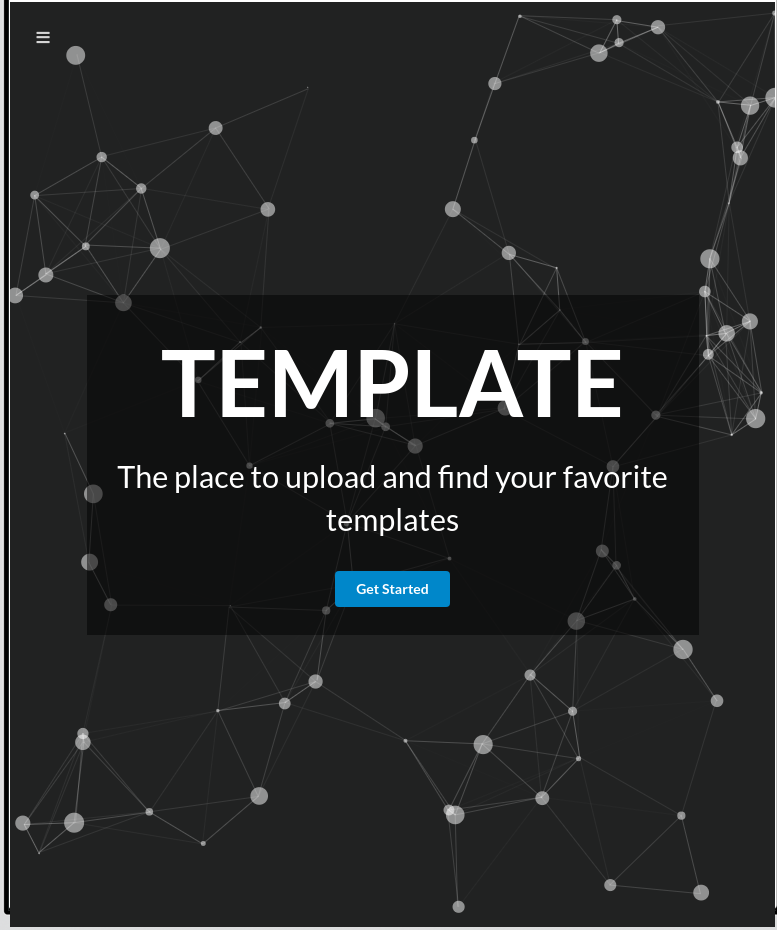
\includegraphics[page=1, scale=0.215]{screenshot/retina.png}
\caption{Ảnh chụp trang home.html trên Retina iPad}
\end{center}
\end{figure}

\begin{figure}[H]
\begin{center}
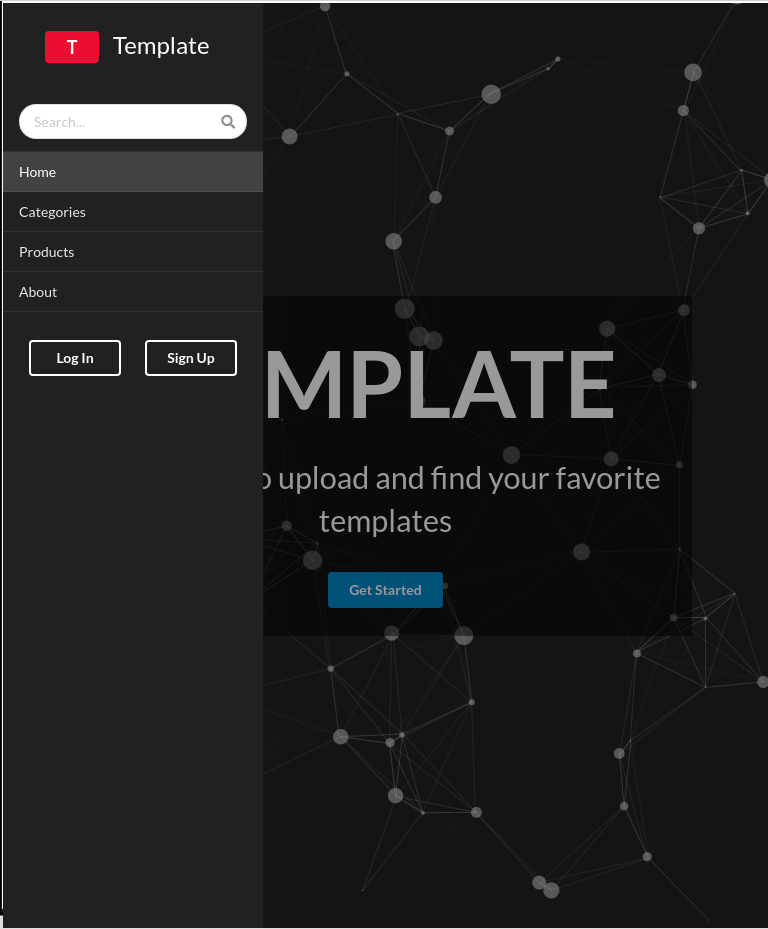
\includegraphics[page=1, scale=0.215]{screenshot/retina2.png}
\caption{Ảnh chụp trang home.html với reponsive menu trên Retina iPad}
\end{center}
\end{figure}


\begin{figure}[H]
\begin{center}
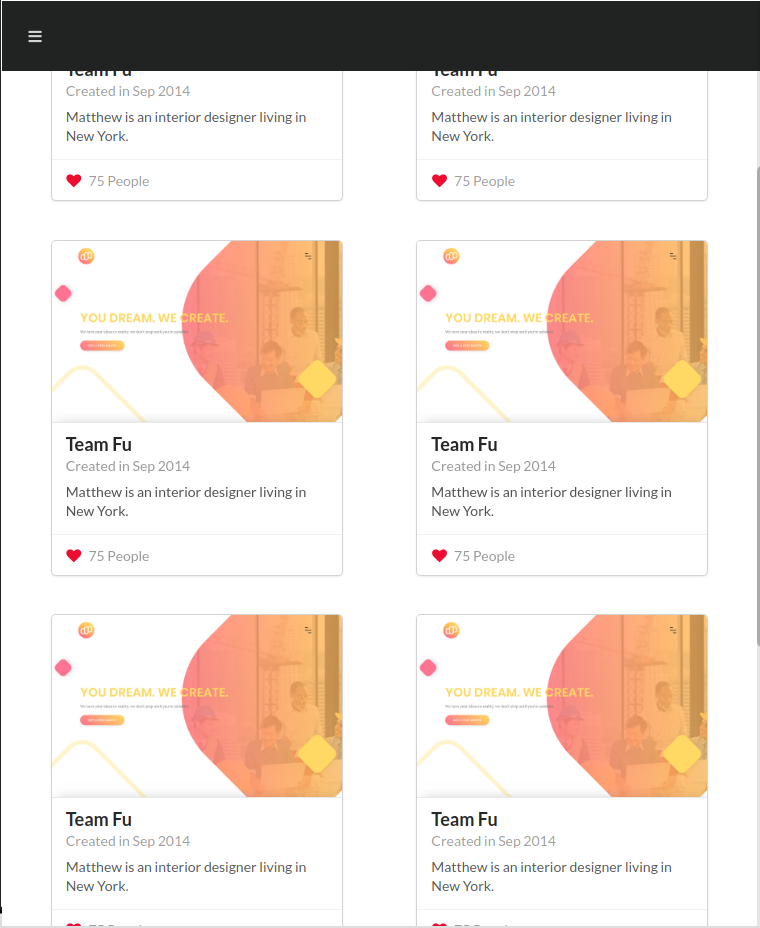
\includegraphics[page=1, scale=0.215]{screenshot/retina3.png}
\caption{Ảnh chụp trang category.html trên Retina iPad}
\end{center}
\end{figure}


\begin{figure}[H]
\begin{center}
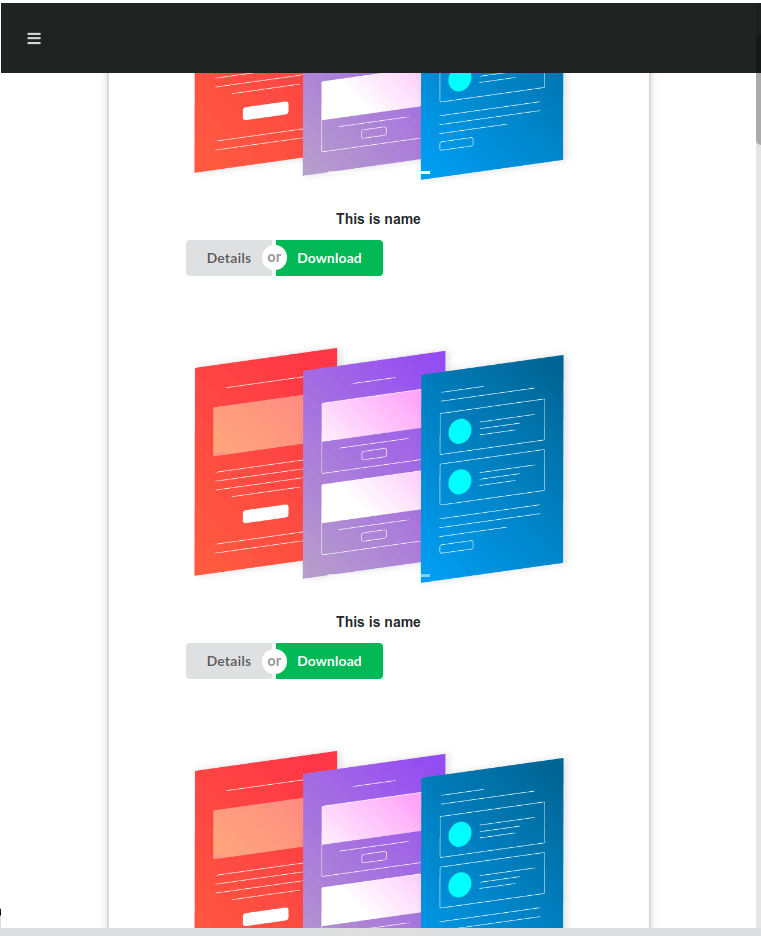
\includegraphics[page=1, scale=0.215]{screenshot/retina4.png}
\caption{Ảnh chụp trang products.html trên Retina iPad}
\end{center}
\end{figure}



\subsection{Hiển thị trên Iphone 5}

\begin{figure}[H]
\begin{center}
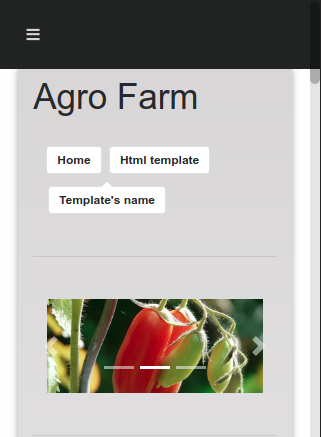
\includegraphics[page=1, scale=0.5]{screenshot/iphone1.png}
\caption{Ảnh chụp trang details.html phần slide trên Iphone 5}
\end{center}
\end{figure}

\begin{figure}[H]
\begin{center}
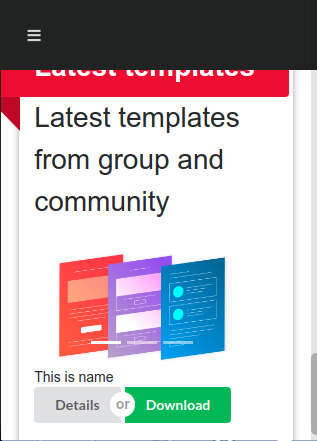
\includegraphics[page=1, scale=0.5]{screenshot/iphone2.png}
\caption{Ảnh chụp trang details.html phần các mục khác trên Iphone 5}
\end{center}
\end{figure}

\begin{figure}[H]
\begin{center}
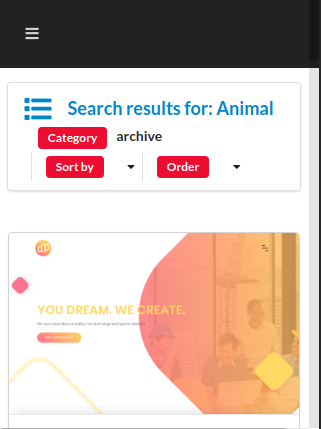
\includegraphics[page=1, scale=0.5]{screenshot/iphone3.png}
\caption{Ảnh chụp trang category.html trên Iphone 5}
\end{center}
\end{figure}

\begin{figure}[H]
\begin{center}
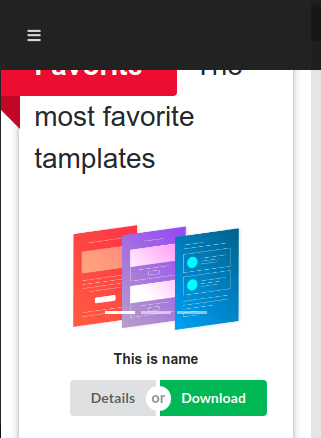
\includegraphics[page=1, scale=0.5]{screenshot/iphone4.png}
\caption{Ảnh chụp trang products.html trên Iphone 5}
\end{center}
\end{figure}


%%%%%%% TONG KET VA KET LUAN %%%%%
\newpage
\section{Tổng kết}
Kết thúc bài tập lớn nhóm đã hiện thực được các giao diện cơ bản của một website chia sẽ Templates. Qua bài tập lớn này nhóm đã rèn luyện được các kỹ năng cần thiết cho lập trình, ngôn ngữ HTML, CSS, JS... sử dụng framework hỗ trợ thiết kế web "Sematic UI".
Nhóm đã  cùng phối hợp với nhau để hoàn thành bài tập lớn lần này, ngoài ra btl này còn tạo điều kiện cho các thành viên trong nhóm có cơ hội học hỏi, trao đổi với nhau. 



%%%% thi%%%  PHAN CONG CONG VIEC %%%%%%
\newpage
\section{Phân công công việc trong nhóm}

\begin{tabu} to 0.7\textwidth { | m{12em} | m{12cm}| }
\hline
 \textbf{Thành viên}& \textbf{Phần việc}\\
\hline
Lê Duy Hiển & \begin{itemize}
\item Lựa chọn framework
\item Xây dựng các thành phần dùng chung
\item Hiện thực các file .html, .css, .js cho trang About
\item Kiểm tra cho trang About
\item Hiện thực các file .html, .css, .js cho trang Home
\item Kiểm tra cho trang Home
\end{itemize}\\

\hline
Trần Quốc Pháp & \begin{itemize}
\item Lựa chọn framework
\item Xây dựng các thành phần dùng chung
\item Hiện thực các file .html, .css, .js cho trang Category
\item Kiểm tra cho trang Category
\item Hiện thực các file .html, .css, .js cho trang Product
\item Kiểm tra cho trang Product
\end{itemize}\\

\hline
Mai Đức Tú & \begin{itemize}
\item Kiểm tra, phân tích trực quan và trải nghiệm người dùng UI/UX
\item Hiện thực các file .html, .css, .js cho trang Login
\item Kiểm tra cho trang Login
\item Hiện thực các file .html, .css, .js cho trang Signup
\item Kiểm tra cho trang Signup
\item Viết report
\end{itemize}\\


\hline
Hoàng Đức Linh & \begin{itemize}
\item Thiết kế giao diện chung cho các trang
\item Kiểm tra, phân tích trực quan và trải nghiệm người dùng UI/UX
\item Hiện thực các file .html, .css, .js cho trang Details
\item Kiểm tra cho trang Details
\item Trao đổi thông tin với các nhóm và làm rõ nội dung, yêu cầu bài tập.
\item Viết report
\end{itemize}
\\
\hline
\end{tabu}

\end{document}

